\chapter{Methodoleg}

Mae'r bennod hon yn desgrifio sut bu prawf geirfa deuaidd yn cael ei lunio yn seiledig ar y pwyntau a amlygwyd yn yr adolygiad llenyddiaeth. Pan fydd agweddau arbennig i ieithoedd yn cael eu mynegu, fel sut i ffynonellu'r geiriau ar lein o eiriadur Llydaweg, deallir y gellir defnyddio'r un dull i greu test mewn iaith arall, pan ni wnaethpwyd o'r blaen.

\section{Ffynonellu'r Allweddiau}
Ar gyfer y prawf geirfa Llydaweg, casgwyd holl gofnodion geiriadur diachronig Llydaweg \href{https://devri.bzh/}{Devri.bzh}, a chynlluniwyd rheolau i dynnu enwau priod ac ôl-ddeiliaid. Gan fod y geiriadur unieithog Meurgorf\footnote{Gweler \url{https://niverel.brezhoneg.bzh/br/meurgorf/}} yn dosbarthu ei gofnodion yn un o dri chategori: aml, cyffredin a phrin, roedd yn bosibl trefnu'r eitemau mewn pedwar categori, y tri blaenorol, a'r eitemau a oedd yn Devri ond nid yn Meurgorf. Dangosir dosbarthiad yr eitemau yn~\ref{tab:breton-types}. Y rhesymau pam y mae cymaint o eiriau yn ymddangos fel pe baent yn absennol yn Devri, yw bod cofnodion Meurgorf yn cynnwys llawer o enwau priod ac ôl-ddeiliaid, yn ogystal â neologismau wedi'u hadeiladu gydag ôl-ddeiliaid cyffredin. Cyfanswm nifer yr allweddi sydd ar gael ar gyfer y prawf oedd 62,169, y rhoddwyd i hanner ohonynt sgôr anhawster rhwng 1 a 3. Ychwanegwyd y cofnodion o Devri na ddarganfuwyd yn Meurgorf at gategori'r tipau prin.

\begin{table}[htbp]
    \centering
    \begin{tabular}{l|r|r|r}
        \textbf{categorïau} & \textbf{ym Meurgorf} & \textbf{yn Devri hefyd} & \textbf{yn unig yn Devri} \\
        \hline
        Aml & 1 108 & 946 & – \\
        Cyffredin & 47 740 & 26 197 & – \\
        Prin & 6 867 & 4 868 & – \\
        Cyfanswm & 55 715 & 32 011 & 30 158 \\
    \end{tabular}
    \caption{Categorïau o eiriau a dynnwyd o Devri (wedi'u hidlo) a Meurgorf}
\end{table}\label{tab:breton-types}

Yn amlwg, nid yw'r categorïau hyn yn berffaith, ond maent yn dal yn gymorth gwerthfawr i gwestiynau anodd graddnodi. Gallai dulliau eraill o gyrchu tipau ac ystodau gwahanol o amlderau ar gyfer ieithoedd eraill gynnwys cyrchu geiriaduron o feintiau gwahanol, gan fydd y geiriau yn y geiriaduriau lleiaf y geiriau amlaf. Mae'r adran ar gychwyn graddio yn dangos sut y defnyddir y graddau cychwynnol hyn. Gellir dod o hyd i'r cod ar gyfer y camau hyn ar GitHub\footnote{Ar gyfer cyrchu geiriau Devri a'u hidlo, gweler y llyfr nodiadau Jupyter hwn: \url{https://github.com/Oktogazh/sudogen/blob/master/1\%20Introduction.ipynb}, ar gyfer yr ystod amlderau, gweler y llyfr nodiadau Jupyter arall hwn: \url{https://github.com/Oktogazh/sudogen/blob/master/locales/br/5\%20Initialization.ipynb}}.

\section{Cynhyrchu'r Llithiau}
\abbrv{LSTM}{Long Short-Term Memory}
\abbrv{RNN}{Recurrent Neural Network}
\subsection{Hyfforddi'r Model}
Am astudiaeth o raddfa'r prosiect hwn, nid yw creu'r geiriau ffug â llaw yn opsiwn. Datblygwyd dulliau gwahanol o greu geiriau ffug yn gyfrifiadurol dros y blynyddoedd, mae'r rhan fwyaf ohonynt yn cadwyni n-gramau a gymerwyd o set ddata hyfforddi o feintiau gwahanol \parencite{new_unipseudo_2023, keuleers_wuggy_2010}. Fodd bynnag, gan fod rhai ieithoedd yn arddangos nodweddion perthnasoedd pellter hir ffônotechtig, megis cysondeb ynganiad mewn ieithoedd Twrcaidd, ystyriwyd nad oedd modelau seiliedig ar n-gramau yn orau ar gyfer creu geiriau ffug tebygol. Am y rheswm hwn, rhoddwyd blaenoriaeth i ddefnyddio Cof Byr Ystod Hir (neu LSTM am Long Short-Term Menmory) \parencite{hochreiter_long_1997}. Bydd y dyluniad yn syml i bobl sy'n gyfarwydd â Rhwydweithiau Niwral Ailadroddus (neu RNN am Reccurent neural Network), ond datblygwyd rhai technegau optimeiddio i gynyddu cyflymder yr hyfforddiant. Gan fod y geiriau yn y set ddata hyfforddi (y allweddi o'r adran flaenorol) o hydoedd amrywiol, mae pop ``batch'' o hyd 1, peth sy'n golygu na allai unrhyw baraleliaeth fod yn bosibl yn ystod hyfforddiant. I osgoi'r broblem hon, cysylltwyd y geiriau mewn cant o linynnau hirach, gyda nodyn llinell newydd a ddefnyddiwyd fel y tocyn arbennig, i ddechrau dilyniant o eiriau, i wahanu pob gair ac i orffen pob dilyniant, gan wneud y dilyniannau hyn yn gryno ac yn ddarllenadwy gan bobl. Cadwyd 15 o'r dilyniannau hyn ar gyfer dilysu a 85 ar gyfer hyfforddiant priodol. Roedd tua 10 dimensiwn mewnosod (i gynrychioli'r cymeriadau) a 180 dimensiwn cudd (i gofio'r patrymau) yn ddigonol i hyfforddi ein model iaith ``orthograffig'' a allai gynhyrchu geiriau ffug o ansawdd da. Mae rhwng 10 a 20 o epocau yn ddigon i gael entropi croes is na 1.8, a diolch i'r dechneg batio a grybwyllwyd uchod, ni chymryd yr hyfforddiant bron yn 10 i 12 eiliad yr epoc. Nodwch, fodd bynnag, nad oedd entropi croes bop tro is yn cael ei gael yn systematig, hyd yn oed gyda'r un hyper-paramedrau, gan fod y proses yn stocastig. Dyma lle mae techneg optimeiddio arall yn dod i'r amlwg, effaith synhwyrol ar gynnydd y ffwythiant colled trwy ail-drefnu'r geiriau mewn trefn wahanol a gwneud dilyniannau gwahanol o'r un geiriau. Yn ffordd, roedd hyn yn ``creu mwy o ddata hyfforddi'' lle mai'r unig bwynt cyffredin rhwng y dilyniannau blaenorol a'r newydd oedd strwythur mewnol y geiriau, a byddai'r cysyltlltiadau rhwng y geiriau ddim yn cael ei hystyried gan fector cudd LSTM. Roedd hyn yn cyfnewid rhai eiriau o'r set dilysu i'r set hyfforddiant, ond gan fod colled ffwythiant y set ddata hyfforddi'n is na chyson ar gyfer pob hyfforddiant, gan ddangos dim arwyddion o ``over-fitting'' hyd yn oed gyda nifer fawr o epocau, roedd hyn yn cael ei ystyried nad oedd yn broblem.

\subsection{Cynhyrchu Geiriau Ffug}
Unwaith y cafwyd model iaith seiliedig ar gymeriad wedi'i hyfforddi gydag entropi croes boddhaol, mae'n barod i gynhyrchu geiriau newydd. Canfuwyd bod tymheredd o 0.7 yn ``bwynt melys'' ar gyfer cydbwysedd da rhwng amrywiaeth a chywirdeb y caracterau a gynhyrchir. Cafodd y pwynt melys hwn ei ganfod trwy edrych ar gyfran y geiriau sy'n dechrau gyda'r llythyren z, yn Llydaweg 1:2000 mathau sy'n dechrau gyda z. Yn amlwg, byddai ieithoedd gwahanol, yn enwedig ieithoedd ag alfabetau eraill angen tymheredd arall.

Gan fod nod y rhwydwaith yw ail-gynhyrchu'r data hyfforddi gyda'r ffyddlondeb fwyaf posibl, bydd yn ceisio cynhyrchu geiriau go iawn. Rhaid hidlo'r geiriau go iawn, a wnaethpwyd mewn dwy ffordd wahanol. Bob tro y cynhyrchwyd gair newydd, pan gynhyrchwyd y caracter llinell newydd, yna cymharir y llinyn caracteriau newydd gyda'r tipau sydd ar gael yn y set ddata hyfforddi, os nad yw yn y set ddata hyfforddi, mae'r gair yn cael ei wirio yn erbyn geiriadur sillafu Hunspell. Dim ond os na chydnabyddir y sillafu yna, mai ychwanegir y gair at set o eiriau ffug a gynhyrchir, gyda gradd uchel o sicrwydd bod y gair yn ddibwys. Mae'r cod ar gyfer cynhyrchu'r geiriau ffug ar gael ar GitHub\footnote{Gweler y llyfr nodiadau Jupyter hwn am fanylion: \url{https://github.com/Oktogazh/sudogen/blob/master/2\%20Training.ipynb}}. Defnyddiwyd y dull hwn i gynhyrchu nifer gyfartal o eiriau ffug â geiriau go iawn.

\begin{figure}[htbp]
    \centering
    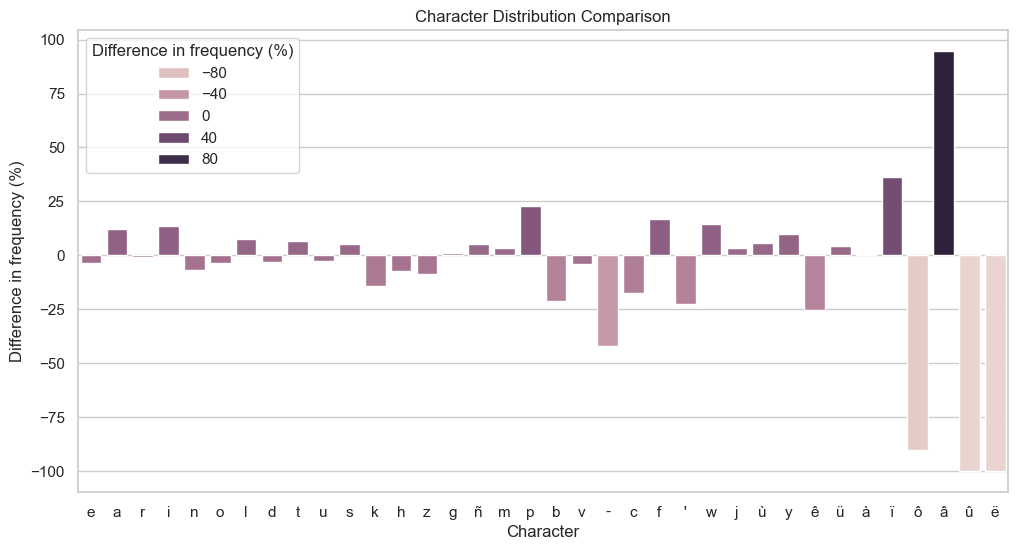
\includegraphics[width=0.8\textwidth]{figures/chars.png}
    \caption{Gwahaniaeth mewn dosbarthiad y caracteriau (geiriau ffug / geiriau go iawn)}
\end{figure}\label{fig:chars}

Gan fod un peth a allai roi geiriau ffug yn ôl yw anghydbwysedd rhai garacteriau yn y geiriau, defnyddir y Ffigur~\ref{fig:chars} i archwilio dosbarthiad y caracteriau trwy'r setiau o eiriau a geiriau ffug. Os yw'r gwerth ar gyfer llythyren benodol yn bositif, mae'n golygu bod y caracter yn cael ei or-ddatblygu yn y set o eiriau ffug, a'r gwrthwyneb os yw'r gwerth yn mynd yn negyddol. Mae'r caracteriau wedi'u trefnu yn ôl amlder, \textit{e} yw'r cymeriad mwyaf cyffredin a \textit{ë} yw'r lleiaf cyffredin yn Llydaweg (a geir unwaith yn unig yn yr eiriau go iawn, ac byth yn yr eiriau ffug, gan hynny'r gwahaniaeth o 100\%). Yn gyffredinol, mae'r' caracteriau yn y geiriau ffug a gynhyrchir yn ymddangos yn gydnaws ag eu dosbarthiad y geiriau go iawn.

\begin{figure}[htbp]
    \centering
    \begin{minipage}{0.45\textwidth}
        \centering
        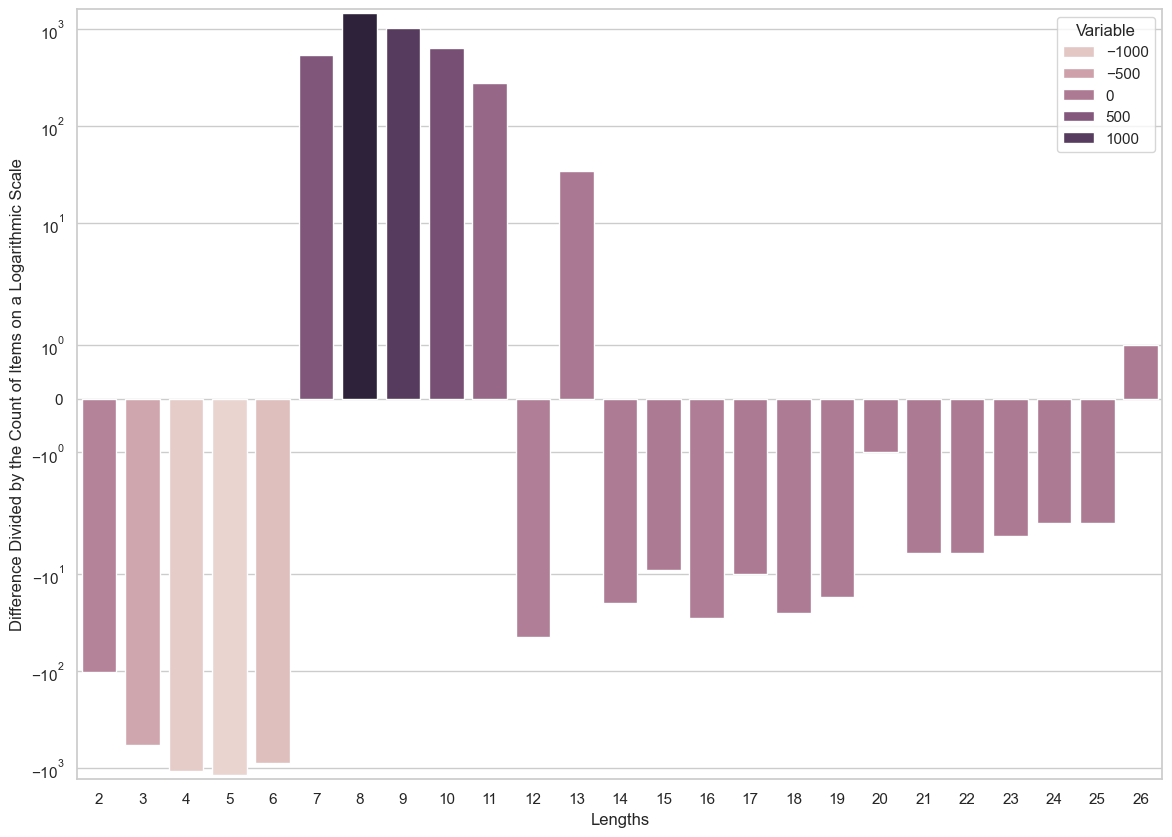
\includegraphics[width=0.8\textwidth]{figures/lengths.png}
        \caption{Gwahaniaeth rhwng y cyfri o eiriau ffug dros eiriau go iawn ar raddfa logarifmig ar gyfer hyd penodol.}\label{fig:lengths}
    \end{minipage}
    \hfill
    \begin{minipage}{0.45\textwidth}
        \centering
        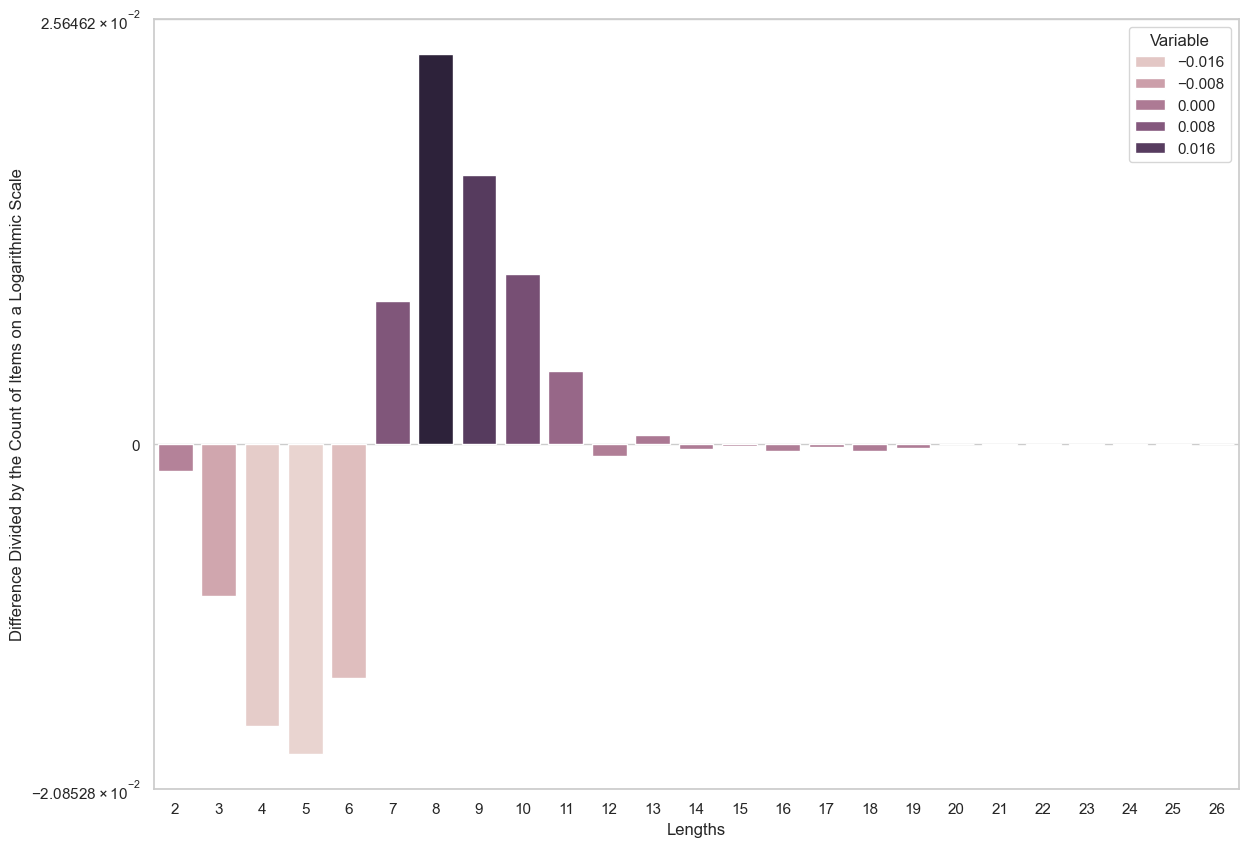
\includegraphics[width=0.8\textwidth]{figures/lengths_divided.png}
        \caption{Yr un gwahaniaeth ag yn~\ref{fig:lengths} wedi'i rannu trwy'r cyfanrif o eitemau i ddod â'r gwahaniaethau yn y cyd-destun o sesiwn brofion.}\label{fig:lengths_div}
    \end{minipage}
\end{figure}

Mae'r ffigurau \ref{fig:lengths} a \ref{fig:lengths_div} yn arbennig o ddiddorol. Gan y gallai'r gwahaniaethau hyd hefyd roi awgrymiadau i'r rhai sy'n cymryd y prawf ar ai yw geiriau gwirion neu ffug. Gellir gweld nad oedd y rhwydwaith wedi cynhyrchu cymaint o eiriau ffug byrion ag yr oedd disgwyl, lle mae eitemau o hyd rhwng 7 ac 11 yn cael eu gor-gyflwyno i raddau. Gallai hyn fod oherwydd bod llai o gymysgeddau o lythrennedd yn bosibl ar gyfer hyd llai, wedi'i gymysgu â'r ffaith bod llawer o'r geiriau posibl eisoes ``wedi'u cymryd'' gan eiriau go iawn. Gan wybod hyn, gellid dylunio rheolau gwahanol wrth gynhyrchu geiriau newydd er mwyn gwneud iawn am y ffenomen hon, fel cynyddu tebygolrwydd ar gyfer nodyn llinell newydd o dan terfyn hyd penodol. Fodd bynnag, gellid ystyried hyn yn or-beiriannaeth. Pan fydd wedi'i leihau i gyfanswm nifer yr eitemau, yn \ref{fig:lengths_div}, gellir gweld bod y rhagfarnau hyd yn amhwysig ac yn annhebygol o roi gwybod am air ffug. Gyda newid uchaf o 1.6\% nid oes ffordd y gallai rhywun sy'n cymryd y prawf ddibynnu ar wahaniaethau hyd i ddyfalu geiriau ffug. Gellir dod o hyd i'r fethodoleg fanwl ar gyfer y ffigurau hyn ar GitHub\footnote{Gweler y llyfr nodiadau Jupyter hwn am fanylion: \url{https://github.com/Oktogazh/sudogen/blob/master/4\%20Testing.ipynb}.}.

\section{Rhoi Gradd Cychwynol i'r Eitemau}
Mae'r diffyg o galibrad cychwynnol yn her enfawr i greu profion sy'n gweithio'n dda. Mae angen i'r prawf gael ei galibradu'n ddigonol fel y gall siaradwyr gyda ystod geirfa gyfyngedig gael eiriau y byddant yn eu hadnabod. Os yw'r rhai sy'n cymryd y prawf yn teimlo eu bod wedi'u diflasu gan sesiwn gyntaf, mae'n annhebygol y byddant yn cymryd y prawf eto, y peth sydd angen i rwystro'r broses galibrad ymhellach. Er mwyn osgoi'r cylch cythreulig hwn, mae angen ``galibrad heb galibrad''. Fel y soniwyd eisoes, mae IAC yn aml yn brin o restrau amlder geiriau, felly ni fydd y dechneg hon yn cael ei datblygu yma, er y gallai fod o ddefnydd i rai ieithoedd.

\subsection{Sut mae'r Graddau Cychwynol yn Effeithio ar Addasolrwydd}
Efelychu gan \textcite{pelanek_applications_2016} a ddangosodd hysbysau sylweddol ar gyfer galibradu anhawster eitemau mewn prawf Elo addasol. Mae'r astudiaeth yn dangos bod yr eitemau yn calibru'n gyflymach mewn system hanner-addasol, yn hytral nâ systemau llawn-addasol neu ddim-addasol. Mae hyn yn herio'r syniad bod system addasol yn defnyddio ansicrwydd i optimeiddio'r elfen wybodaeth a gafwyd o bob eitem. Ysywaeth, nid yw'r astudiaeth yn rhoi manylion am ddosbarthiad cychwynnol anhawster yr eitemau. Yn enwedig, os yw'r eitemau i gyd wedi'u gosod i'r un anhawster cychwynnol, bydd prawf llawn-addasol yn cael ei ragfarnu i ddewis yr eitemau a ddewiswyd eisoes, gan fod yr eitemau heb eu dewis yn dal i fod yn eu gwerth cychwynnol, cudd mewn math o dan gwerth nad yw'n debygol o gael ei gyrraedd gan y rhai sy'n cymryd y prawf wrth iddynt symud oddi wrth y norm. Efallai mai dyma pam y gwelwyd gwelliant wrth ychwanegu rhywfaint o haprwydd at y broses ddewis eitemau.

\subsection{Bagu Modwlo}
Gellir defnyddio'r syniad grwpio'r eitemau o amgylch gwerthau i mewn math gwahanol i fuanu'r calibradu. Ond yn hytrach na grwpio'r holl eitemau o amgylch yr un gwerth, mae'n bosibl grwpio'r eitemau o amgylch lluosrif o werth penodol. Mae hyn yn gadael bylchau yn y dosbarthiad anhawster cychwynnol, a fydd yn cael eu llenwi wrth i'r broses galibrad fynd yn ei blaen. Mae hyn yn gwneud y dosbarthiad anhawster cychwynnol yn fwy amrywiol, gan ganiatáu i'r system llawn-addasol ddewis eitemau sydd wedi agosi 'w gradd cywir, ond hefyd rhai nad ydynt wedi'u calibri eto, ers llai o'r rhain. Bydd hyn yn cynyddu'r amrywiaeth o eitemau a ddewiswyd, gan ganiatáu i'r broses galibrad fynd yn ei blaen yn fuan. Bydd hyn hefyd yn lleihau'r tebygolrwydd y bydd y rhai sy'n cymryd y prawf yn cael eu diflasu gan gael yr un math o eitemau drosodd a throsodd. Fel y soniwyd eisoes, mae clystyrau rhy bell i ffwrdd o'i gilydd yn gallu diraddio'r broses galibrad ei hun. Mae system o'r fath yn symud o dipyn i beth o system seiliedig ar gyfran, lle mae'r sgôr yn dibynnu ar y nifer o eitemau a adnabuwyd yn iawn, i system sy'n seiliedig ar raddfa logistaidd lle mae'r sgôr yn dibynnu ar y gallu i adnabod eitemau gyda anhawster penodol. Dyma a enwasom ``bagu modwlo'' (modulo clustering) neu ``fagu mewn ffa''. Deallir mai ar gyfer brawf o gymaint o eitemau i gael eu calibri a chyn lleied o bobl i'w cymryd ag sydd mewn cyd-destun IAC, ni fydd y prawf byth yn un neu'r llall yn llwyr, ond system seiliedig ar gyfran sy'n symud yn barhaus tuag at raddfa logistaidd, lle'r rhan fwyaf wedi'i chalibrio yw'r ystod sy'n cynrychioli lefel is o fedrusrwydd. Dim ond trwy system addasol lawn sy'n defnyddio'r dechneg bagu modwlo y mae'r system hon yn bosibl. 

\begin{figure}
    \centering
    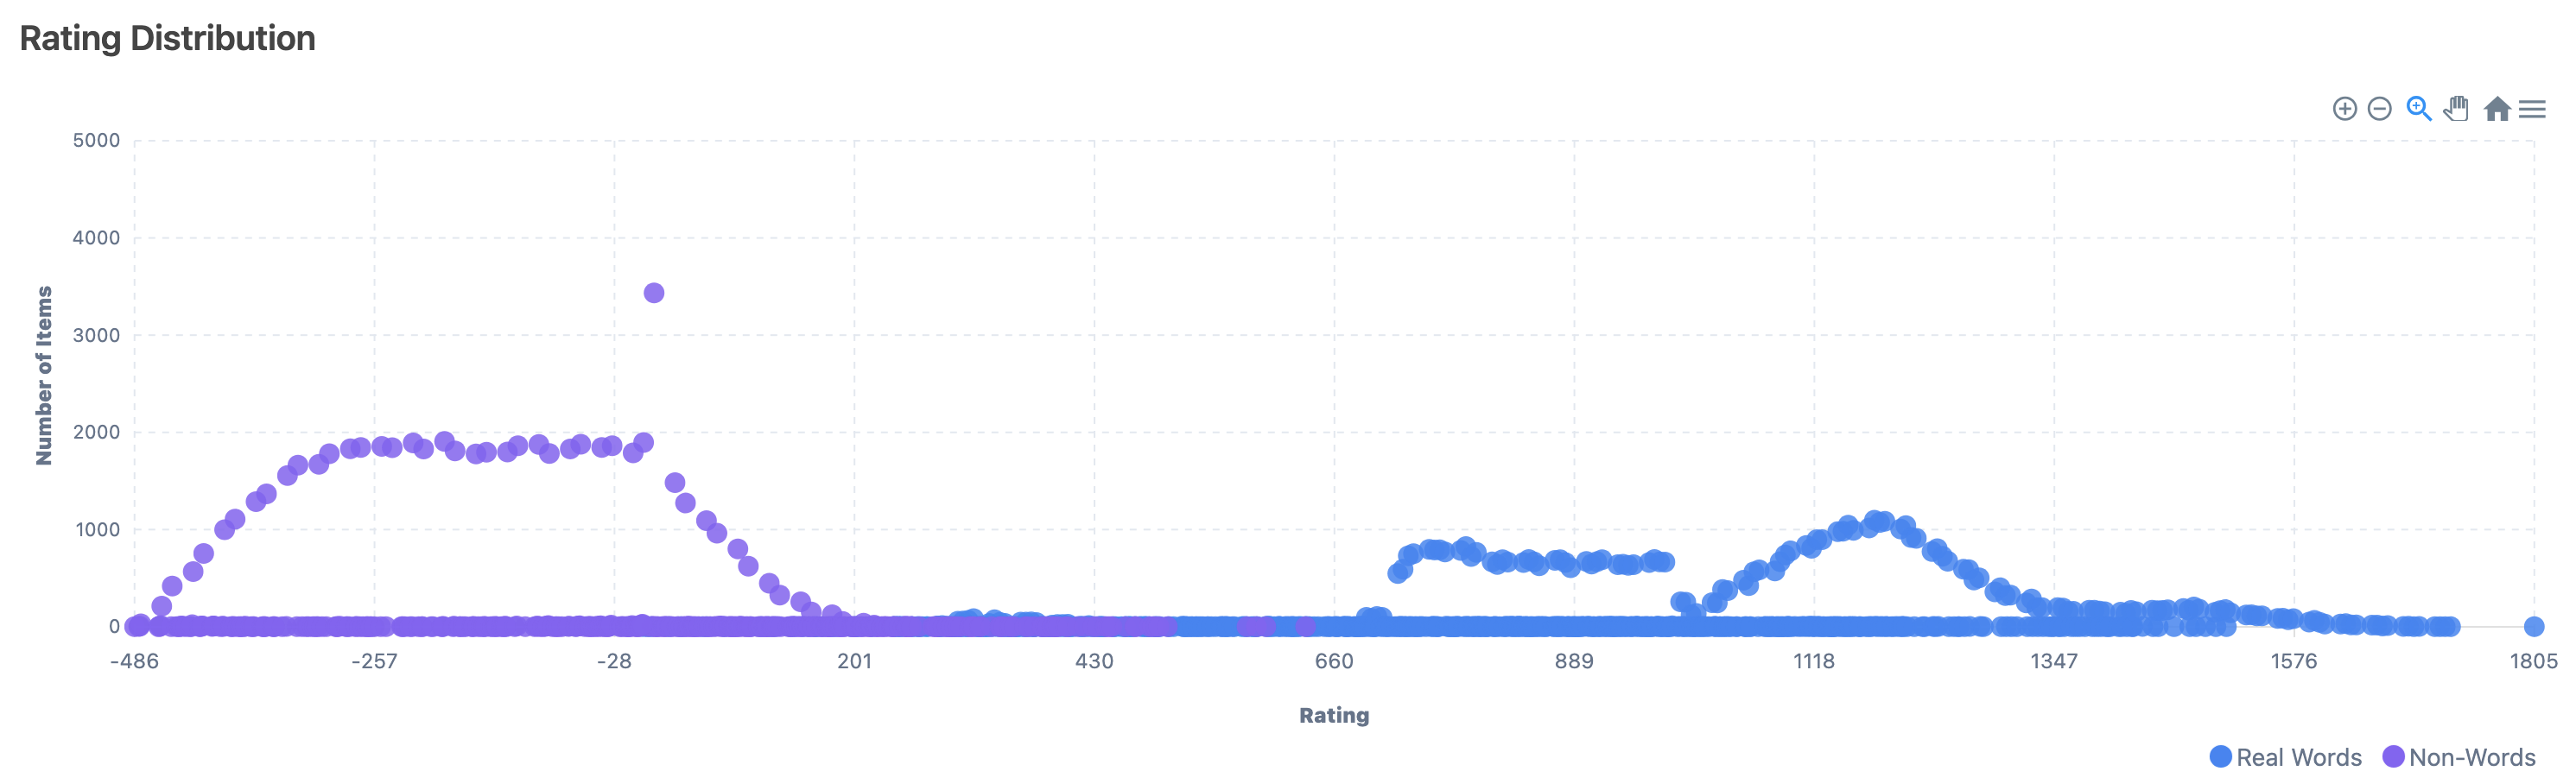
\includegraphics[width=0.9\linewidth]{figures/distribution-items.png}
    \caption{Dosbarthiad yr eitemau ar ôl ddechrau'r proses calibri}
    \label{fig:distribution}
\end{figure}

\subsection{Gradd Cychwynol yr Llithau}
\abbrv{CAC}{Cyfran o Atebion Cywir (neu PC am Proportion of Correct Answers)}
Gan ddisgwylir y llithiau, neu eiriau ffug, i gael eu adnabod yn llai aml na'r allweddi, disgwylir bydd eu sgôr yn disgyn. Os yw sgôr yr allweddi (geiriau go iawn), wedi'i capio uwchben sero, er mwyn dangos bod sgôr prawf uwchben sero yn symbolaidd o wybodaeth iaith nad yw'n sero, gall sgôr y llithiau fod yn negyddol. Fel arall, byddai'r llithiau'n grwpio ar raddfa sero. Am y rhesymau hyn, penderfynwyd rhagbaratoi'r galibrad a rhoi sgôriau negyddol ar hap i eitemau nad ydynt yn eiriau go iawn, sy'n golygu bod gwahaniaeth yn y sgôr cyfartalog rhwng yr allweddi a'r llithiau. Cyn dechrau sesiwn, yn ystod dewis yr eitemau, mae'r gwahaniaeth hwn yn cael ei gywiro trwy ychwanegu 'r gwahaniaeth rhwng y cyfartaleddau hyn at y sgôr presennol.  Mae hyn yn effeithio fel ``cosbi'' mwy difrifol am adnabod gair ffug na'r cynnydd mewn sgôr sy'n gwobrwyo am adnabod gair go iawn. Felly byddai twyllwr sy'n honni'n gyson ei fod yn adnabod pob eitem yn wynebu gostyngiad llym yn ei sgôr, yn hytrach na sgôr sefydlog.

Mae'r ffigur \ref{fig:distribution} yn rhoi cynrychiolaeth o ddosbarthiad yr eitemau trwy sgôriau. Gellir gweld y clystyrau yn hedfan dros yr eitemau sydd mewn proses galibrad. Mewn dosbarthiad mwy wedi'i galibrad, byddai'r ddwy linell yn uno'n un. Fel y gallwn ei weld yn yr un ffigur, mae'n edrych fel bod y proses galibrad wedi mynd yn ei flaen ar gyfer y geiriau o'r ystod amlder uchaf (y llwmp glas bach islaw sgôr 500), sef union yr ystod o brawfwyr lle na fyddai prawf sy'n seiliedig ar gyfran o atebion cywir (CAC) yn addas, ac y mae angen raddfa logistaidd fel system sgorio Elo.

\section{Byrhau'r Rhestr o Eitemau}
O'r adran hon ymlaen, symudwn i ffwrdd o gwestiwn yr eitemau i ganolbwyntio ar fecanwaith y prawf ei hun. Cafodd y prawf ei gyflwyno ar blatfform gwe sydd ar gael yn agored heb ofyn i ddefnyddwyr greu cyfrif\footnote{Gweler \href{https://leksis.bzh}{https://leksis.bzh}}. Disgwylir i sesiwn brawf ddefnyddio dim ond rhan fach o'r eitemau sydd ar gael, ac felly daeth y syniad o fyrhau'r rhestr o eitemau ar gael. Yn hytrach na samplu eitemau'n ar hap o'r rhestrau o eitemau, a fyddai'n dewis bron yn unig eitemau nad ydynt wedi'u calibri, mae'r prawf yn dewis eitemau trwy sgôr unigryw, sy'n disgyn siawns cael geiriau nid aseswyd trwy sesiwnau blaenorol. Felly, mae'r eitemau nad ydynt yn cael eu dewis yn ystod y broses fyrhau yn eitemau sydd wedi'u grwpio ar eu sgôr modwlo cychwynnol. Byddai gan yr eitemau hyn siawns fach iawn o gael eu dewis heb y broses fyrhau hon, oherwydd mewn gosodiad addasol, maent yn perthyn i glystyrau o sawl can o eitemau. Mae'r broses fyrhau hon felly'n cynyddu perfformiad sesiwn brawf heb bwysleisio ansawdd y prawf. Gan fod yr eitemau'n cael eu cymysgu cyn cael eu dewis trwy sgôr unigryw, nid yw'r eitemau sydd wedi'u byrhau byth yn union yr un peth (yn enwedig y rhai nad ydynt wedi'u dewis eto), gan gyfrannu at unigrywiaeth pob sesiwn. 

Pan ailddechreuir sesiwn newydd yn uniongyrchol ar ôl gorffen un, mae'r un rhestr o eitemau yn cael ei defnyddio eto heb yr eitemau a gynnigwyd yn y sesiwn gynt, gan ganiatáu i'r rhai sy'n cymryd y prawf gymryd y prawf eto heb weld yr un eitemau dwy waith.

\section{Y Sesiwnau}
\begin{figure}
    \centering
    
\includegraphics[width=0.5\linewidth]{figures/screenshot-redadeg.png}
    \caption{Sgrinlun o rwyngwyneb y brawf yng nghabol sesiwn brawf Lydaweg.}
    \medskip
    \small
    Mae'r gair ``redadeg'' Llydaweg yn enwog oherwydd ras bi-flwydd sy'n digwydd ar draws y wlad. Byddai llawer o bobl nad ydynt yn siaradwyr yn dal i adnabod y gair hwn, sy'n gwneud yr ateb o'r eitem hwn yn enghraifft o'r trydydd rheswm a roddwyd ar gyfer diweddaru sgôr am y rheswm anghywir: nid yw sgôr yr eitem yn cyfateb i'w radd profi go iawn. Disgwylir i'r broblem hon ddiflannu'n gyflym wrth i fwy o bobl ateb y prawf.
\end{figure}\label{fig:screenshot}

\subsection{Diweddaru Sgôr y Defnyddwyr a Hyd y Sesiwn}
Mae diweddaru sgôr y defnyddwyr yn digwydd yn real-time ac mae'r sgôr bresennol yn cael ei dangos iddynt. Mae dwy ffordd i golli pwyntiau, trwy beidio â chydnabod gair go iawn neu trwy gydnabod geiriau ffug. Nid yw peidio â chydnabod llithiau yn dylanwadu ar y sgôr ac yn unig mae cydnabod geiriau go iawn sy'n cynyddu'r sgôr.\\
Mae'r sylfaen logarhythmig ar gyfer y cynnydd yn 10, gyda ffactor lledaenu o 400, fel mewn gwyddbwyll er mwyn cadw'r sgôr yn ddarllenadwy gan bobl. Mae'r sgôr bob amser yn cael ei dangos iddynt. Defnyddir y ffwythiant ansicrwydd (gweler y hafaliad~\ref{eq:uncertainty-function}), gyda $a=100$ a $b=0.05$. Mae hyn yn golygu bod cydnabod cywir gair go iawn yn dod â 47 pwynt y tro cyntaf y cyflwynir gair go iawn i'r defnyddiwr, a thua 8 pwynt ar ôl 100 o weithiau, hynny yw, hanner canlyniad y ffwythiant ansicrwydd oherwydd bod y tebygolrwydd o atebion cywir bob amser yn amgylchynol 50\%. Fodd bynnag, mae'r ffwythiant ansicrwydd wedi'i chapio i 20 pwynt er mwyn cynnal cynnydd cyson ar gyfer perfformwyr gwell. Mae cyflymder y cynnydd sgôr yn bwysig gan fod hyd sesiwn brawf yn cael ei bennu gan y sgôr bresennol, gweler isod yr hafaliad sy'n penderfynu ar nifer y geiriau go iawn i'w hateb cyn i sesiwn ddod i'w phen.

\begin{equation}
    f(x)=10 + x/14
\end{equation}\label{eq:length-function}

Lle mae $f(x)$ yn rhoi nifer y geiriau go iawn i'w hateb, a $x$ yw'r sgôr bresennol. Felly, mae sesiwn brawf yn dechrau gyda 10 eitem i gydnabod, ac mae'r nifer hon yn cynyddu wrth i'r sgôr gynyddu. Mae hyn yn golygu bod sesiwn brawf yn para o leiaf tua 20 eitem (10 gair go iawn a tua 10 gair ffug), ac yn cynyddu'n raddol wrth i'r sgôr gynyddu. Mae hyn yn sicrhau nad yw perfformwyr ``gwael'' yn disgwyl mynd trwy sesiwn brawf hir. Gan ystyried sgôr o tua 146 (a gafwyd ar ôl dim ond tri ateb cywir yn olynol), ni fyddai'r sesiwn brawf yn para llawer mwy na 22 eitem a ddangosir (11 gair go iawn ac oddeutu tua 11 gair ffug). Felly, byddai'r prawf yn defnyddio tri gair go iawn i godi i sgôr y prawfwr, a byddai'r 9 eitem sy'n weddill yn cael eu defnyddio i ddarganfod pa eiriau y mae dysgwr lefel 150-tybiedig yn eu hadnabod ac yn eu hanwybyddu.

Pan atebir y gair go iawn olaf, dangosir y sgôr terfynol i'r defnyddiwr, a anfonir gan y platform canlyniadau'r brawf i'r gronfa ddata. Mae sgôr yr eitemau a ddefnyddiwyd yn ystod y diwrnod yn cael ei diweddaru bob dydd at hanner nos.

\subsection{Dewis yr Eitemau mewn Sesiwn}
Pan ddechreuir sesiwn brawf, mae'r program yn dewis un o'r ddwy restr o eitemau, allweddi neu llithiau, ar hap. Os yw'r rhestr a ddewiswyd yn allweddi, yna mae'r eitemau gyda'r sgôr agosaf at sgôr bresennol y prawfwr yn cael eu dewis. Fel y soniwyd yn gynharach, pan ddewisir y rhestr o llithiau, yna ychwanegir y gwahaniaeth rhwng cyfartaledd sgôr y llithiau a chyfartaledd sgôr yr allweddi at sgôr bresennol y prawfwr. Os yw sgôr bresennol y prawfwr yn 500 a bod y gwahaniaeth rhwng cyfartaledd sgôr yr allweddi a chyfartaledd sgôr y llithiau yn 600, yna bydd y prawf yn chwilio am eitem (gair ffug) gyda sgôr o -100.

Am resymau perfformiad, nid yw'r prawf yn aros am ateb i ddod o hyd i'r eitem nesaf. Cyn gynted ag y bydd eitem newydd yn cael ei harddangos ar y sgrin, mae'r prawf yn cyfrifo'r sgôr nesaf ar gyfer y ddau ganlyniad, atebion da neu ddrwg, ac yn dewis dau eitem yn seiliedig ar y newidiadau hyn yn y sgôr. Mae'r system hon, ynghyd â'r ffaith bod rhestrau'r eitemau'n cael eu byrhau cyn dechrau sesiwn, yn sicrhau trosglwyddiad llyfn a di-dor ar ôl pob ateb.

\section{Diweddaru Sgôr yr Eitemau}
Mae gradd yr eitemau yn cael ei diweddaru'n ddyddiol, yn seiliedig ar ganlyniadau manwl y prawf a storir yn y gronfa ddata yn ystod y dydd blaenorol. Mae'r system yn dilyn diweddariad system raddio Elo, hefyd, yn seiliedig ar y ffaith bod y diweddariadau hyn yn anghydamserol, gallai rhywun ddychmygu systemau eraill i ddiweddaru'r radd. Er enghraifft, dylai gair go iawn gyda gradd gychwynnol o 100 nad yw'n cael ei gydnabod gan brawfwr gyda sgôr terfynol o 500 gael ei gynyddu o leiaf i 500. Rhaid bod ffyrdd gwell o ddiweddaru radd eitem benodol, ond yn y pen draw, arweiniodd y pwysau amser at ddiweddariad syml ar sail y gwahaniaeth rhwng y rhagfynegiad a'r sgôr go iawn wedi'i luosi â ffactor K o 20 (yn lle swyddogaeth ansicrwydd). Nodwch, fodd bynnag, fod sgôr ddisgwyliedig eitem yn cael ei chyfrifo mewn swyddogaeth o'r sgôr terfynol o'r sesiwn brofion, nid y radd ar y foment yr oedd yr eitem yn cael ei hateb.

Gan ddisgwylir y bydd y geiriau ffug a gynhyrchwyd o lefelau credibilidad amrywiol, mae'n cael ei dderbyn y gall rhai geiriau ffug fod yn hollol annhebygol ac y gall eraill fod yn eiriau ystyrlon, gwirioneddol nad oedd erioed wedi'u hychwanegu at eiriaduron. Byddai'r credibilidad amrywiol hon yn cael ei hystyried yn broblem yn y rhan fwyaf o arbrofion ieithyddol cymhwysol, gan y byddai disgwyl i'r un gradd o nonsens ddod o bob gair ffug, ond mae'n anochel pan gynhelir eitemau gan y degau miloedd. Drwy ddiweddaru gradd y geiriau ffug, mae'r prawf hwn yn cydnabod y ffaith nad yw pob gair ffug wedi'i greu'n gyfartal, ac y gallai eiddo annisgwyl o eiriau ffug ganiatáu i bobl gydnabod y rhain fel eiriau gwirioneddol neu anwirioneddol. Mae hyn yn golygu y gallai geiriau ffug y mae eu gradd yn cynyddu i bwynt lle byddai mwy na hanner y rhai sy'n cymryd y prawf yn eu hystyried yn eiriau gwirioneddol (gan gynnwys siaradwyr mwy datblygedig) yn cael eu hadnabod a'u symud o un rhestr i'r llall. Nid yw'r prawf yn darparu mecanweithiau i wneud hyn eto, heblaw am lawrlwytho ffeil JSON yr eitemau gyda'u gradd bresennol a gweithredu'r ffeil yn llawol cyn ei llwytho i'r cais gwe eto. Ond mae'r posibilrwydd y gallai geiriau ffug a gynhelir wneud synnwyr i'r rhai sy'n cymryd y prawf yn cael ei ystyried yn dda, ac mae'r broblem yn cael ei datrys o leiaf yn rhannol gan y dyluniad presennol, gan y bydd eitemau a gydnabyddir yn aml yn ymddwyn yn wahanol i'r norm a'u dangos yn llai a llai diolch i'r system diweddaru.

\section{Ychwanegu Ieithoedd Newydd}
Ar adeg ysgrifennu, ychwanegwyd tair iaith arall i'r platfform, Cymraeg, Wcreineg a Ffrangeg. Yn seiliedig ar dreialon cynnar o'r prawf Lydaweg, gwnaethpwyd rhai newidiadau i weithdrefn cychwyn sgôr yr eitemau. Yn gyntaf, roedd y sgôr cychwynnol ar gyfer y ddwy rhestr, allweddi a'r llithiau wedi'u gwasgaru o fewn yr un ystod o sgôriau, rhwng 0 a 2000, gan yr un sail modwlo o 5. Roedd hyn oherwydd sylweddoli bod y gwahaniaeth mawr yn y sgôr cyfartalog (rhwng allweddi a llithiau) a ddisgrifir uchod efallai'n rhy fawr ac nad oedd y dirywiad yn sgôr bresennol y prawfwyr yn adlewyrchu eu canlyniadau go iawn, fel y byddai'n cael ei esbonio yn yr adran nesaf. Felly roedd sgôr y llithiau wedi'i wasgaru'n gyfartal rhwng 0 a 2000, tra bod sgôr yr allweddi wedi'i wasgaru rhwng 0 a 1000 yn seiliedig ar is-ystodau sy'n seiliedig ar restrau amlder, tra byddai gweddill yr allweddi wedi'u gwasgaru ar hap rhwng 1000 a 2000. Mae nifer yr eitemau yn yr ystod 0-1000 yn amrywio yn seiliedig ar y rhestrau amlder sydd ar gael ar gyfer iaith benodol, ond deallir mai dim ond rhan fach o'r allweddi fyddai'n dod i fod yn yr ystod hon. Mae hyn yn creu gwahaniaeth yn y sgôr cyfartalog rhwng yr allweddi a'r llithiau, er gwahaniaeth mwy rhesymol. Gellir dod o hyd i fanylion y cod a ddefnyddiwyd ar gyfer iaith benodol eto ar GitHub\footnote{Dewch o hyd i fanylion iaith benodol trwy eu cod iaith IETF yn y cyfeiriadur hwn \url{https://github.com/Oktogazh/sudogen/tree/master/locales}, gyda'r ffeil 4.ipynb yn gyfrifol am gychwyn sgôr yr eitemau.}

\section{Atborth}
\abbrv{LLM}{Large Language Model}
Gan fod yn hanfodol i'r broses galibrad gael llawer o bobl yn cymryd y prawf, datblygwyd dwy strategaeth i gynnydd y ymrwymiad. Yn gyntaf, y gallu i rannu eu sgôr gyda dolen i'r prawf. Yn ail, promt manwl ar gyfer model iaith mawr (LLM) sy'n integreiddio canlyniadau'r prawf, sydd wedi'i gynllunio i roi adborth adeiladol trwy ddysgu ystyr y geiriau nad ydynt wedi'u hadnabod. Mae'r wers bersonol a rhyngweithiol hon yn canolbwyntio ar y geiriau gyda'r sgôr isaf, gan ofyn i'r defnyddiwr fwrw ymlaen i adeiladu brawddegau gan ddefnyddio'r geiriau newydd. Ar ôl hynny mae'n cynnig mynd yn ddyfnach i ddatblygu'r gair hwn trwy ddangos cynnwys amlgyfrwng sy'n defnyddio'r geiriau, neu i barhau i ddysgu am y geiriau go iawn eraill nad ydynt wedi'u hadnabod, uwch eu sgôr. Gellir copïo a gludo'r promt i LLM hoff y defnyddiwr, neu, os yw'r porwr yn caniatáu hynny, ei rannu'n uniongyrchol gyda'r ap LLM gyda'r API navigator.share()\footnote{Gweler \url{https://developer.mozilla.org/en-US/docs/Web/API/Navigator/share}}. Gellir dod o hyd i fersiwn y promt ar adeg ysgrifennu yn yr Atodiad \ref{pnd:Promt Dadansoddi}, ynghyd ag enghraifft o ateb gan GPT-5.
\begin{figure}[htbp]
    \centering
    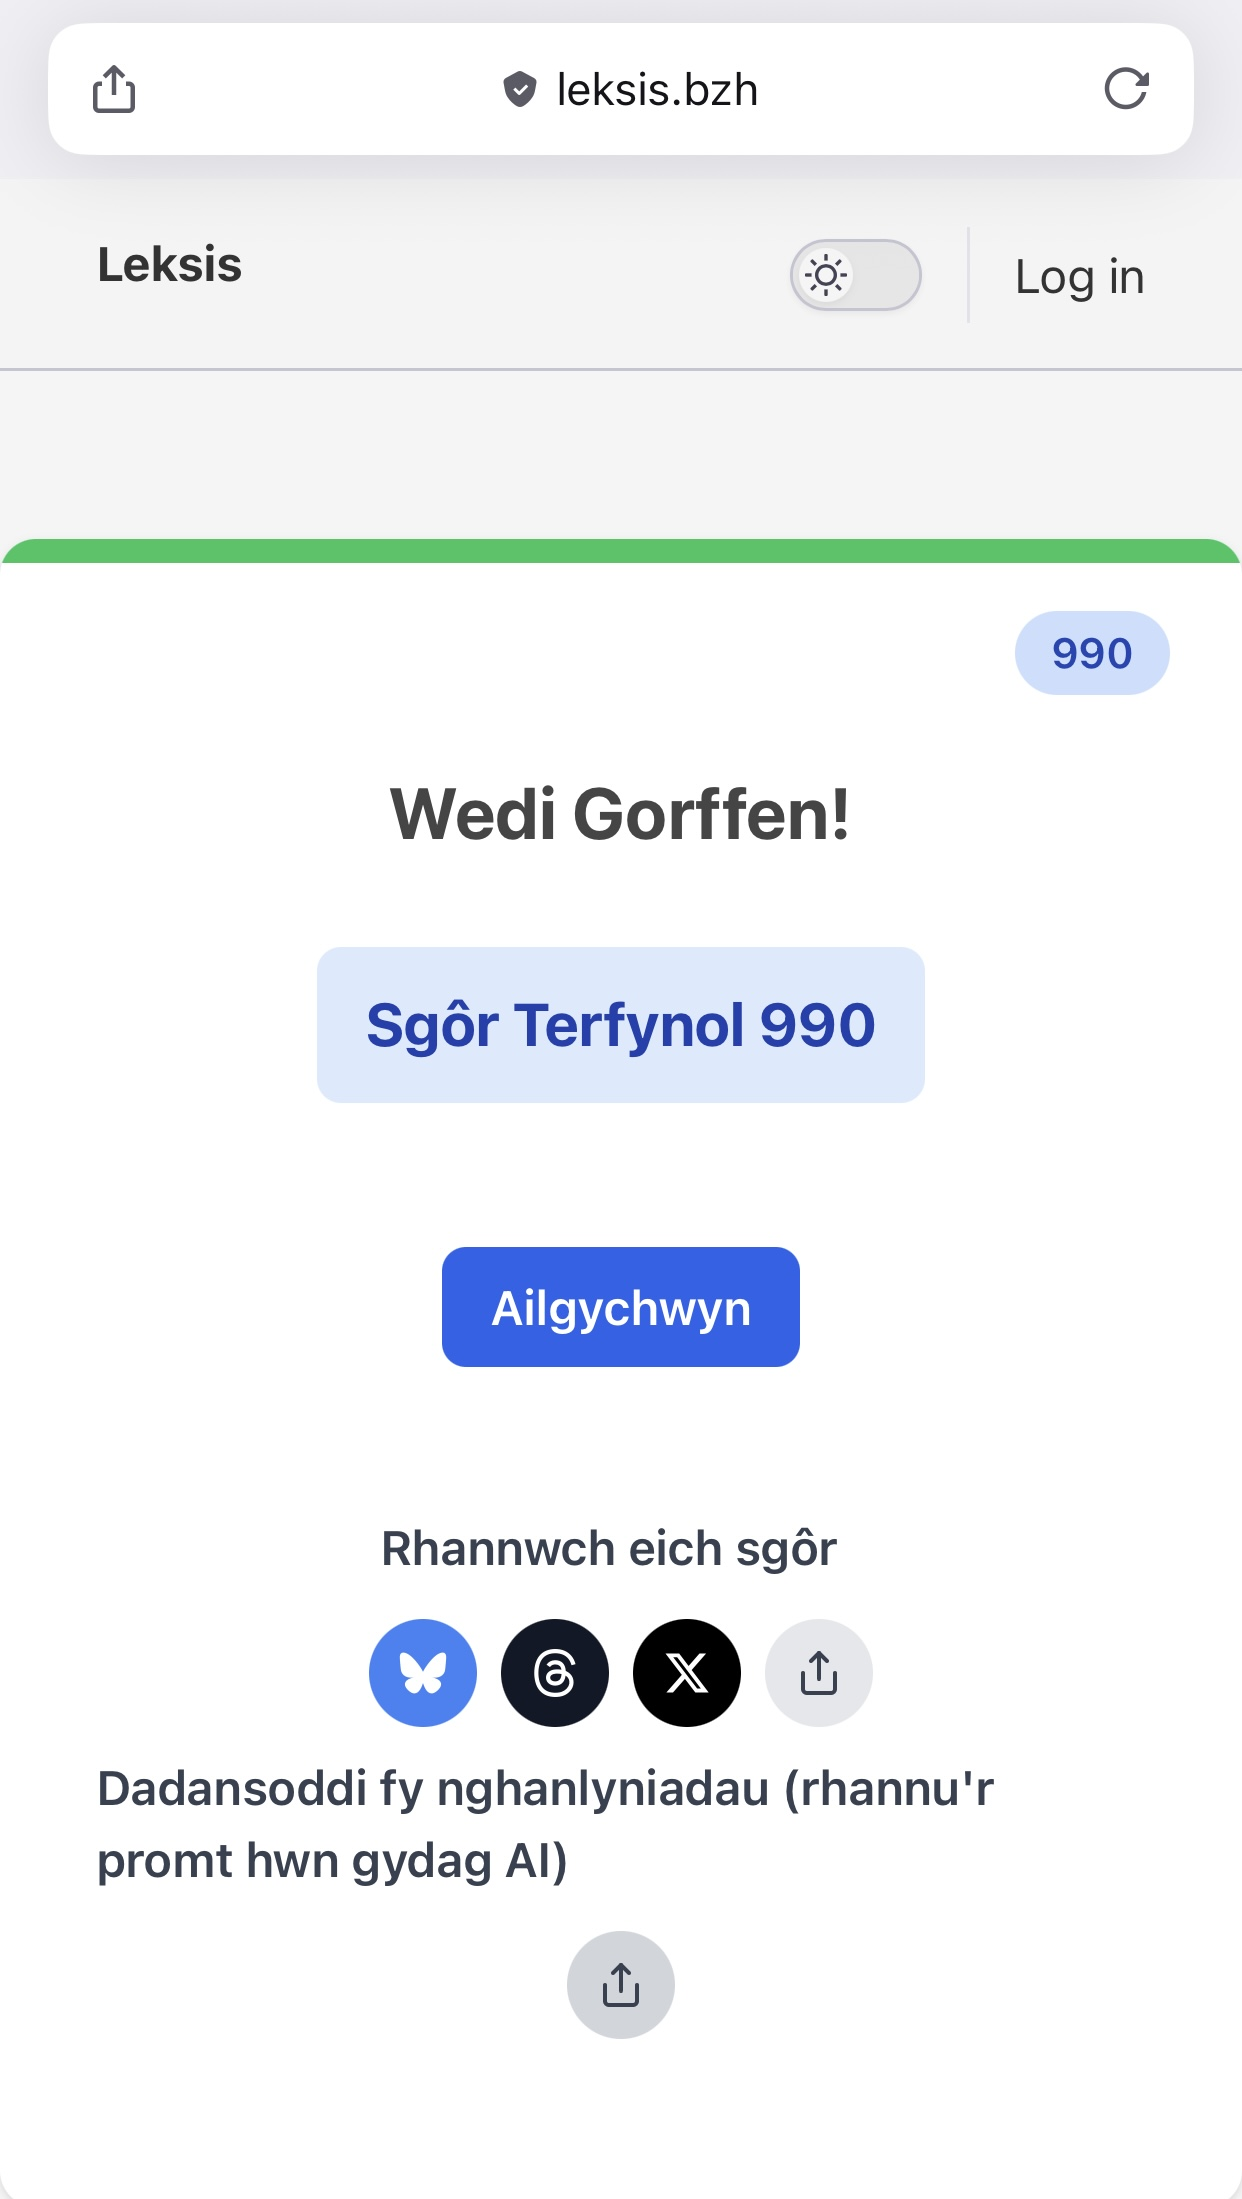
\includegraphics[height=0.7\textwidth]{figures/end-screen.jpg}
    \caption{Sgrinlun o'r sgrin olaf ar ôl cwblhau sesiwn brawf, gyda'r opsiynau i rannu canlyniadau neu gael adborth gan LLM.}
\end{figure}\label{fig:endscreen}

\section{Dilysu'r Prawf}
\subsection{Construct Validity and Design Choices}
In the domain of psychometrics, when the traits measured are latent, it is essential to test the tests, a process called validation. Validation theory is dominated by principles established by \textcite{messick_validity_1987} who unified different aspects of validity, thus simplifying previous approach to the matter.\ \textcite{borsboom_concept_2004} on his end, attempted to simplify construct validity discution a step further by incisting on key concepts in the scientific method, ontology, meaning, causation. Borboom pointed out that much of the construct validity discussion was more about the validation processes than the validity of the constructs themselves. His argument was, consciously or not, integrated in~\cite{kane_validating_2013}. This paper introduced an argument-based approach to validation, where a given test must be proposed along a set of claims, which must be tested individually.

As far as construct validity is concerned, the first half of the literature review showed how a LDT vocabulary test can be used to indirectly measure other constructs of proficiency. The concern of this dissertation is not the validation of the construct itself, but the validation of the calibration methodology and the scoring system. This includes the following:

\begin{enumerate}
  \item The use of a logarithmic scale as a knowledge model, to represent the difficulty rating of the items.
  \item The use of frequency lists for the ratings initialisation.
  \item The use of the ``beans'' modulo clustering technique to increase the chances of encountering better calibrated items and obtain meaningful results without a full calibration.
\end{enumerate}

The first point, the use of a logarithmic scale, by its statistical nature, is valid. At least in a context where a large enough number of tests are taken to calibrate the items. The real issue with the current framework is its ability work without an extensive calibration. This is why the focus of the validation process must be on the two other design choices. To validate these design choices, we must make inferences on how the test would behave under certain condition. To make sure that the test would capture small variation in vocabulary level, these two inferences must be verified:

\begin{enumerate}
  \item \textbf{Reliability}: People taking the test several times in a row will obtain a similar score. Below 1000, the items initial rating are random values within some range. In French the 1000 most frequent items are randomly rated between 0–400, the 1000 to 2000 most frequent words between 400–500 and so on. By ``similar'' we mean that the scores stay within such a range.
  \item \textbf{No ceiling effects}: People with different vocabulary level should not get stuck in the same score range. Three critical ranges can be identified: around 0, where beginner would end up with a null score despite some vocabulary knowledge; around 1000, where the ratings cease to be defined based on frequency and start to become truly random; around 2000, where all fluent speakers would know enough words to have a positive ratio along the 1000–2000 range.
\end{enumerate}

The most complete way to verify these inferences would be to run an integration test. Take a group of beginners in a year-long intensive course for adults and collect the results at taking the test every single week. Inspect how fast the students progress, where they stagnate, be it at similar periods in time (around holidays) or at similar score level, which would indicate a ceiling effect.

Such an integration test cannot be made in the span of time covered by a dissertation. But the early development of tests for a few language may still bring insights on the matter. Especially regarding reliability, it is possible to inspect anonymous test results to see how stable the predictions become as a test session is carried on. If the score is accurate, the chance of recognising real words are around 50\%, which is a falsifiable claim. However, validating the reliability of the test on some ranges does not inform on the potential ceiling effect. A broader study is required for this.

\subsection{Clarifications and Results Interpretation}
Before going further, there is a need to clarify a few points in order avoid a misinterpretation of the results. Especially, it is understood that a growth in the test-taking skill should not be generalized blindly. That it can interpreted as proficiency growth only as long as the learning activity consist of a real use of the language, where the vocabulary is learned within the use of grammatically correct sentences. Taking the test repeatedly may make the test taker being better at taking the test without improving their proficiency proper. Finally, it is understood that tests score cannot be universally interpreted in a similar way, 1500 in the Welsh test and the French test cannot be worth the same thing for the following reasons:
\begin{enumerate}
  \item Socio-linguistic differences make it difficult to find equivalence in the idea of fluency.
  \item The number of items is different for different languages, the initialisation of the items rating is based on frequency lists of different lengths. This leads to different scores at equivalent vocabulary sizes.
  \item Considering that a wide-spread usage of the tests change the ratings dramatically, the rating of the items will have a tendency to cluster around the level of the test takers demographics. If many very fluent people take one test, the ratings value will be devaluated. If many beginners take a test, the items rating will be subject to an inflationary effect.
\end{enumerate}

None of the aspects cited above are seen as a problem for the intended goal of the test. The test aims at measuring the dynamics, the speed at which the learners acquire language over periods of weeks and months. For this purpose only reliability and the absence of ceiling effects are needed.

\subsection{Validation Protocol}
The goal of an adaptive system is to reach the point of highest uncertainty. We can use the last real words in the test sessions see how likely they are to be recognised. If the recognision rate of the last item in the test sessions is close to 50\%, it demonstrates that the test finds items that are right at ``the breaking point'' mentioned above. For this, we can use the p-value from a binomial test to understand how normal the distribution is. We can then inspect the deviation from the 50\% landmark to look for early signs of ceiling effects in different ranges.
